\iffalse
	前言:
		魔改自西工大的简历模板:https://www.overleaf.com/latex/templates/npu-cv/mncqzxhvfzrx,不过已经面目全非了。西工大的那个模板也是参考自一个祖传的模板,以及https://github.com/LeyuDame/BNUCV/tree/main 上的BNU的latex简历模板中的代码。
        基本相当于完全重构了一遍代码,只有一部分变量名还有注释继承自老代码。

        ———— 本简历由 21级药学院 小红(某正经温迪厨) 开发 ————
		
        每个章节的格式都能混着用,顺序都可以变,只是给了个例子。
        比如你找工作,可以把技能那部分往前挪。
        比如你竞赛经历很多,你就往前挪。
        比如你觉得“其他”有点多余,就删了。

        LaTeX排版就是很整齐,强迫症狂喜。


        如果你用overleaf可以忽略下面内容,但如果你用的TexLive等等,就要阅读以下文字:
        注意要用XeLaTeX编译链进行编译,且要进行三次编译才能显示照片。问就是LaTeX的锅。
		vscode+latex的话,配置的json中"latex-workshop.latex.recipes"添加:
		{
            "name": "XeLaTeX*3",
            "tools": [
                "xelatex",
                "xelatex",
                "xelatex"
            ]
        }
		即可使用三次XeLaTeX编译。
		LaTeX+VScode的配置https://www.zhihu.com/column/p/166523064。
        记得要三次XeLaTeX编译!!!
        记得要三次XeLaTeX编译!!!
        记得要三次XeLaTeX编译!!!
        这个很重要,所以说三遍!

        你可以试试两次的,好像某些环境两次编译也能显示图像,但最好还是三次编译。
\fi

\documentclass[11pt]{article}
% 五号字美观不伤眼。

\usepackage{ctex}
\usepackage{xltxtra}
\usepackage{bookmark}
\usepackage{hyperref}
\hypersetup{hidelinks}
\usepackage{url}
\urlstyle{tt}
\usepackage{multicol}
\usepackage{xcolor}
\usepackage{calc}
\usepackage{graphicx}
\usepackage{tikz}
\usetikzlibrary{calc}
\usepackage{fontspec}
\usepackage{xeCJK}
\usepackage{relsize}
\usepackage{xspace}
\usepackage{fontawesome}
\usepackage{titlesec}
\usepackage{enumitem}
\usepackage{siunitx}
\usepackage{amssymb}
\usepackage{tabularx}
\usepackage{multicol}
\usepackage{fontspec}

%%%%%%%%%%%%%%%%%%%%%%%%%%%%%%%%%%%%%%%%%%%%%%%%%%%%%%%%%%%%%%%%%%%%%%%%%%%%%%%%%%%%%%
%    !!!!!!!! 这部分内容,在对LaTeX语法完全不熟悉的情况下不要随便改,已经尽量调整成舒服的程度了 !!!!!!!!
%%%%%%%%%%%%%%%%%%%%%%%%%%%%%%%%%%%%%%%%%%%%%%%%%%%%%%%%%%%%%%%%%%%%%%%%%%%%%%%%%%%%%%

% 一些小设置,参考自https://github.com/LeyuDame/BNUCV/tree/main
\CJKsetecglue{}							            % 取消中文字符与数字之间的间隔
\protected\def\Cpp{{C\nolinebreak[4]\hspace{-.05em}\raisebox{.28ex}{\relsize{-1}++}}\xspace}	% 这是个更好看的C++写法,你直接写C++的话,+号会很大,可以使用\Cpp来代替
\setlength{\parindent}{0pt}							% 取消全局段落缩进
\pagenumbering{gobble}								% 取消页码显示
%\setlist{noitemsep}									% 禁用列表中项目之间的额外垂直间距,但保留列表周围的间距
%\setlist{nosep}										% 禁用列表中项目之间的额外垂直间距及列表周围的间距

\newcommand{\Anewpage}
{
    \newpage
    \begin{tikzpicture}[remember picture, overlay]
		\node[anchor=north, inner sep=0pt](header) at (current page.north){
			
\includegraphics[width=\paperwidth]{images/h-new.png} % 大括号里面可以改相对路径替换页首图片
		}; %页首图片
		\node[anchor=west](school_logo) at (header.west){
            \vspace{-0.3em}
			\hspace{0.5cm}
			
\includegraphics[width=0.25\textwidth]{images/CPU-logo.png}
		}; %页首校徽
		\node[anchor=east](school_name) at(header.east){
			\textcolor{white}{\textbf{\NameFont \zihao{4}\school}} 
			\hspace{0.5cm}
		}; %页首学院名
	\end{tikzpicture}
    \vspace{0.6cm}
	% 页脚,联系方式
	\begin{tikzpicture}[remember picture, overlay]
		\node[anchor=south, inner sep=0pt](footer) at (current page.south){
			
\includegraphics[width=\paperwidth]{images/f.png} % 大括号里面可以改相对路径替换页脚图片
		};
        % 联系方式
        \node[anchor=center] at(footer.center){\contact};
	\end{tikzpicture}
	% 背景
	\begin{tikzpicture}[remember picture, overlay]
		\node[opacity=0.1] at(current page.center){
			
\includegraphics[width=0.7\paperwidth, keepaspectratio]{images/CPU-Blank.png}
		};
        \node[anchor=south, inner sep=0pt](footer) at ([yshift=0.871cm]current page.south){
			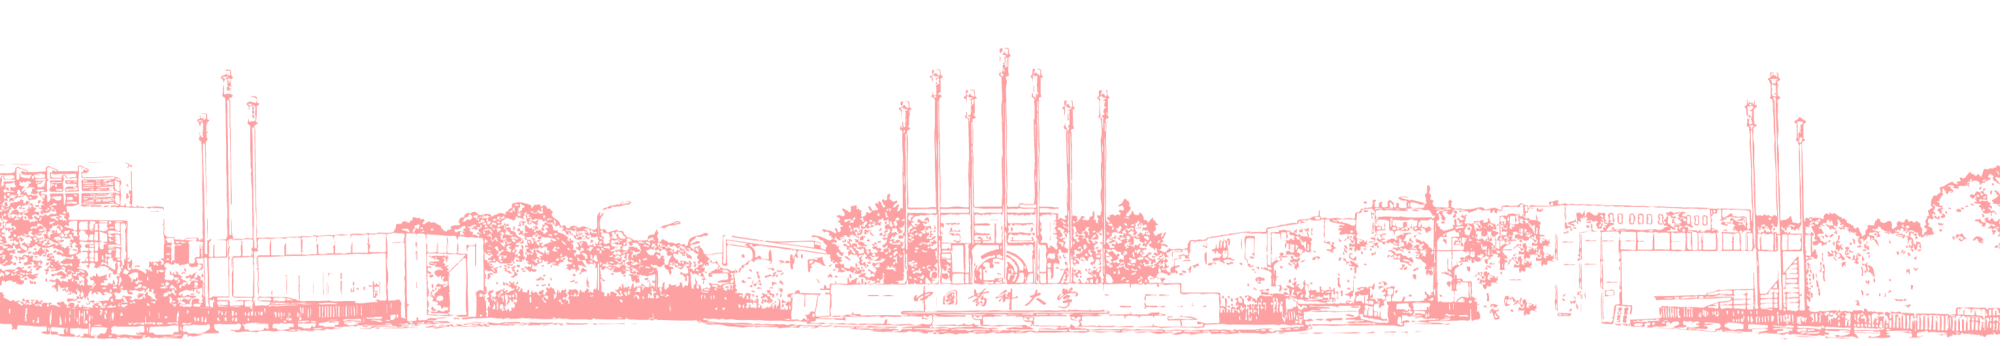
\includegraphics[width=\paperwidth]{images/Bottom.png} % 大括号里面可以改相对路径替换背景图片
		};
	\end{tikzpicture}
}
% 主题色
% 药大蓝
\definecolor{CPU_Blue}{RGB}{36,72,158}

% 不太刺眼的药大红
\definecolor{CPU_Red}{RGB}{133,19,33}

%%%%%%%%%%%%%%%%%%%%%%%%%%%%%%%%%%%%%%%%%%%%%%%%%%%%%%%%%%%%%%%%%%%%%%%%%%%%%%%%%%%%%%
%    !!!!!!!! 以下部分可在充分了解LaTeX语句情况下改动数字(如有任何困难可以交给Deepseek修改),实现压缩简历至一页的效果。 !!!!!!!!
%%%%%%%%%%%%%%%%%%%%%%%%%%%%%%%%%%%%%%%%%%%%%%%%%%%%%%%%%%%%%%%%%%%%%%%%%%%%%%%%%%%%%%

\setlist[itemize]{leftmargin=1em, labelsep=0.35em}
\setlist[enumerate]{leftmargin=1em, labelsep=0.35em}

\titleformat{\section}					    % 将原标题前面的数字取消了
  {\zihao{3}\bfseries\raggedright} 		      % 字体改为小三号,bold,左对齐
  {}{0em}                      			  % 可用于添加全局标题前缀
  {}                           			  % 可用于添加代码
  [{\color{CPU_Red}\titlerule}]            % 标题下方加一条线
\titlespacing*{\section}{0cm}{*1.25}{*1.25}	% 标题左边留白,上方1.25倍,下方1.25倍

\titleformat{\subsection}				    % 将原二级标题前面的数字取消了
  {\zihao{-4}\bfseries\raggedright} 		      % 字体改为四号,bold,左对齐
  {}{0em}                      			  % 可用于添加全局二级标题前缀
  {}                           			  % 可用于添加代码
  []
\titlespacing*{\subsection}{1.6cm}{*1.2}{*1.2}% 二级标题左边留白,上方1.2倍,下方1.2倍

\usepackage[ % 页面大小与页边距,按需求调整
	a4paper,
	left=1.2cm,
	right=1cm,
	top=1.2cm,
	bottom=1.2cm,
	nohead
]{geometry}

\renewcommand{\CJKglue}{\hskip 0.05em}% 中文字符间距

\setmainfont[]{Times New Roman} %原模板用的微软雅黑,但我觉得新罗马体更符合科研宝宝体质。

\setCJKmainfont[]{SimSun}% 中文字体 宋体

\newCJKfontfamily\NameFont{YanKai.ttf}[% 名字和学院名换一种好看的字体。
  Path = fonts/,
  Extension=.ttf
]

% 这里把正文的行间距调成1.5倍了
\linespread{1.5}

% 这里把表格的行间距调成1倍了
\renewcommand{\arraystretch}{1}



%%%%%%%%%%%%%%%%%%%%%%%%%%%%%%%%%%%%%%%%%%%%%%%%%%%%%%%%%%%%%%%%%%%%%%%%%%%%%%%%%%%%%%
%    !!!!!!!! 以下部分一定要修改到你自己的情况 !!!!!!!!
%%%%%%%%%%%%%%%%%%%%%%%%%%%%%%%%%%%%%%%%%%%%%%%%%%%%%%%%%%%%%%%%%%%%%%%%%%%%%%%%%%%%%%


\newcommand{\school}{ 药学院 | \setmainfont[]{Times New Roman}\textbf{School of Pharmacy}}% 学院
% 也可以不写英语

% 联系方式
% 邮箱确实是我的,有任何修改建议可以直接给我发送邮件。
\newcommand{\contact}
{
    \small              % 换了更小的字号
    % \footnotesize       % 这比上面的小一号
    %\scriptsize         % 这比上面的再小一号
    \textcolor{white}
    {
        \faEnvelope \qquad \href{mailto:xiaohong@stu.cpu.edu.cn}{xiaohong@stu.cpu.edu.cn}    % 邮箱,前面的超链接可以直达邮箱软件
        \hspace{4em}    % 这里可以调间距
        \faWechat \qquad XiaoHong               % 不知道谁的微信
        \hspace{4em}    % 这里可以调间距
        \faPhone \qquad 114-1919-8810                  % 不知道谁的手机号
        \hspace{4em}    % 这里可以调间距
        %\faGithub \quad \href{https://github.com/xxxx}{https://github.com/xxxx}         % github,也可以换成你本人博客地址
    }
}

%%%%%%%%%%%%%%%%%%%%%%%%%%%%%%%%%%%%%%%%%%%%%%%%%%%%%%%%%%%%%%%%%%%%%%%%%%%%%%%%%%%%%%
%    !!!!!!!! 这里开始就是正文了 !!!!!!!!
%%%%%%%%%%%%%%%%%%%%%%%%%%%%%%%%%%%%%%%%%%%%%%%%%%%%%%%%%%%%%%%%%%%%%%%%%%%%%%%%%%%%%%


\begin{document}
	\Anewpage 
    \vspace{-2.4em}
    % 自定义了生成新页的命令,每次另开新页都要加这个
    % 当然对于简历来说我觉得两页完全够了。
    %%%%%%%%%%%%%
	% 以下部分是个人信息
    %%%%%%%%%%%%%
    \begin{figure}[h]
        % 左半边,信息,比例占行宽87%,可以自己调
        \begin{minipage}[c]{0.25\textwidth}
             \NameFont \zihao{1}巴巴托斯  %名字很长的话建议把字号调小, -1表示小一号,2表示二号字,以此类推
        \end{minipage} % 名字占25%
        \begin{minipage}[c]{0.03\textwidth}
             \hfill \rule{1.5pt}{1.8cm}
        \end{minipage} % 垂直线(宽度 1pt,高度 1.8cm)
        \begin{minipage}[c]{0.56\textwidth}
            \begin{tabularx}{\linewidth}{XX}
                性别:男 & 出生日期: ??.6.16\\
                籍贯:北方大陆蒙德 & 政治面貌:七十二魔神 
            \end{tabularx}
        \end{minipage} %这段是你的个人信息,占59%
        % 右半边,照片,比例占行宽12%,可以自己调
        % images/Venti.png 替换成你证件照的路径。
        \begin{minipage}[c]{0.12\textwidth}
            
\includegraphics[width=\linewidth]{images/Venti.png}
        \end{minipage}
        % 尽量留至少1%的间距,不然会换行
        \begin{minipage}[c]{0.99\textwidth}
            \zihao{-4}\textbf{求职意向: }\hspace{1em}巡演吟游诗人,谢绝任何需要坐班的工作。
        \end{minipage}
    \end{figure}
    \vspace{-1.6em}
    %%%%%%%%%%%%%
	% 教育背景
    %%%%%%%%%%%%%
    	% \faGraduationCap这类\fa开头的都是font awesome里的logo,想换成其他logo的话,可以看一下附带的fontawsome.pdf,自行替换。
		% \section{\makebox[\widthof{\faGraduationCap}][c]{\color{CPU_Red}{     这里!    }}\quad 标题}
    \section{\makebox[\widthof{\faGraduationCap}][c]{\color{CPU_Red}{\faGraduationCap}}\quad 教育背景}
            \subsection{ 中国药科大学 \qquad 药理学 | 博士 \hfill 2019年 - 2025年}
            \qquad 不知道啊我就一小本科生,怎么知道博士毕业的在这里会写啥。

            \subsection{ 北陆魔神学院 \qquad 古典诗歌创作 | 本科 \hfill 前1644年 - 前1638年}
            \vspace{-0.8em}
            \begin{tabularx}{\textwidth}{XXX}
                \textbf{GPA: 4.75/5.0 }& \textbf{加权平均分: 95.52/100}  & \textbf{综测排名: 1/64} 
            \end{tabularx}
            大学在校认真学习,知识掌握充分。\textbf{连续六年排名在专业第一并获得校优秀学生奖学金。}撰写《风与牧歌之城考据》,复原蒙德古地名体系;开发「千风乐章」吟唱法,开创诗歌与元素力共鸣理论。

            \textbf{主修课程及分数:}
            \vspace{-0.8em}
            \begin{table}[h]
                \centering
                \zihao{5}
                % 这里建议左边填字数少的课程
                \begin{tabular}{ p{2cm} p{\widthof{100}} p{3cm} p{\widthof{100}} p{3.5cm} p{\widthof{100}} p{4cm} p{\widthof{100}}}
                    文字学 & 100 & 古代文化概论   & 98 & 元素导论 & 91 & 提瓦特古文字学 & 98 \\
                    音韵学 & 98 & 文献学概论    & 96 & 蒙德文学批评史 & 94 & 提瓦特哲学史大纲   & 97 
                \end{tabular}
            \end{table}
            \vspace{-1.2em}
    %%%%%%%%%%%%%
    % 竞赛经历(找导师也可能看中这个,因为代表了一定实践能力,但是尽量对口吧,不要运动会都写进去了)
    %%%%%%%%%%%%%
    \section{\makebox[\widthof{\faGraduationCap}][c]{\color{CPU_Red}{\faTrophy}}\quad 竞赛获奖}
    \vspace{-1.2em}
    \begin{table}[h!]
        \begin{tabularx}{\textwidth}{p{\widthof{1234567890年}}Xp{\widthof{团队全国二等奖\&个人全国三等奖}}}
            前1642年 & 提瓦特酒业协会品鉴赛       & \textbf{金奖(提瓦特一等奖)}        \\
            前1641年 & 第三届「风花节」诗歌大赛         & \textbf{北陆二等奖}        \\
            2021年 & 第四届 ETO 成员三体运动计算方案建模竞赛          & \textbf{F奖(特等提名奖)}
        \end{tabularx}
    \end{table}
    %%%%%%%%%%%%%
    %这部分是科研成果,写你发的论文或者书刊
    %可以修改为实习经历那个样子,在下面写你的研究Abstract
    %%%%%%%%%%%%%
    \section{\makebox[\widthof{\faGraduationCap}][c]{\color{CPU_Red}{ \faClipboard}}\quad 科研成果}
    \vspace{-1.2em}
    \begin{table}[h!]
        \begin{tabularx}{\textwidth}{p{\widthof{选一个最长的期刊名}}Xp{\widthof{第八十八作者}}}
            \textbf{非人物种健康} & 特瓦林睡眠障碍干预:风琴声波与泪滴结晶协同治疗方案 & \textbf{通讯作者}        \\
            \textbf{J.PoemCom.Mon} & The Disappearance of Ancient Mongolian Warsong and Rise of Popular Folk Music:Discussion on the Deconstruction of Art Forms by Freedom.& \textbf{第一作者}\\
        \end{tabularx}
    \end{table}
    %%%%%%%%%%%%%
    %这部分是实习经历,一般写各种公司啊什么的,大创可以写到后面
    %%%%%%%%%%%%%
    \section{\makebox[\widthof{\faGraduationCap}][c]{\color{CPU_Red}{\faFlask}}\quad 实习经历}
    % 小技巧,老师想看的重点加粗,比如商科类的一般更想看到数字,工科类的更想看到技术
    \subsection{\parbox{\widthof{天使的馈赠酒馆}}{西风骑士团}\qquad 风魔龙危机应对课题组 \quad 特别行动顾问 \hfill 2025.2 - 2025.5}
    \qquad 指导荣誉骑士完成“用泪滴结晶哄龙入睡”等非常规战术设计“用暴风眼反推能量核心”方案,危机解除后\textbf{被琴团长授予“摸鱼救世主”称号}
    % 给一个正经的例子:\qquad 学习\textbf{MTT、CCK-8、PCR、WesternBlot、流式细胞技术、共培养实验}等基本药理学实验,负责\textbf{筛选潜在肿瘤治疗或肾脏保护作用的活性化合物}。参与\textbf{实验动物日常饲养和基因型鉴定}。
    \subsection{\parbox{\widthof{天使的馈赠酒馆}}{天使的馈赠酒馆}\qquad 驻场吟游诗人 \hfill 2023.2 - 2025.1}
    \qquad 凭《野猪公主》系列故事换取蒲公英酿,创下\textbf{单日拉动酒水销量500\%记录}。\textbf{首创开发“诗与酒”捆绑销售模式,}被老板迪卢克评为“最想赶走但又舍不得的营销鬼才”
    %%%%%%%%%%%%%
    \Anewpage%新建一页用这条指令
    %%%%%%%%%%%%%
    %%%%%%%%%%%%%
    %这段科研经历可以写大创
    %%%%%%%%%%%%%
    \section{\makebox[\widthof{\faGraduationCap}][c]{\color{CPU_Red}{ \faBalanceScale}}\quad 科研经历}
    %\subsection{\parbox{\widthof{  如果想要冲齐这里写上你最长的项目名称  }}{  这里写你的项目  } \qquad \qquad 这里看你想写啥了\quad 团队负责人当然要强调 \hfill 日期}
    % 在研的也能写
    % 课程大作业也能写,但是不要标明是大作业就行
    % 一个例子,别真写金工实习做榔头
    \subsection{\parbox{\widthof{大国工匠-论锤子是怎么炼成的}}{APTX4869药物研发} \qquad \qquad 国家级大创优秀结题\quad 第一负责人 \hfill 2023.1 - 2025.1}
    \qquad  主要负责药物的\textbf{前期研发,中期亲自试药和后期的投毒计划部署}与主要执行人员。成功将著名侦探\textbf{工藤新一}变成小孩摸样。药物的研发成功让\textbf{150万人}收益,最终盈利\textbf{3000万元}。
    \subsection{\parbox{\widthof{大国工匠-论锤子是怎么炼成的}}{大国工匠-论锤子是怎么炼成的} \qquad \qquad 校级创新工程实践\quad 主要技术负责人 \hfill 2023.1 - 2023.2}
    \qquad 对古代中国工匠制作锤子的历史、工艺和技术进行深入研究,包括原材料的选择、工具的制作、锤子的设计和锻造工艺等方面。结合现代工艺技术和设计理念,探索如何将古代工匠的技艺与现代制造工艺相结合,以提高锤子的性能、品质和设计。通过实际制作锤子的过程,验证理论和技术的可行性,并对制作过程中的关键环节进行深入分析和总结。
    %这个例子太复杂了,编不下去,索性抄NPU的模板吧。
    %%%%%%%%%%%%%
    % 技能特长,上面写很多的话,这里就随便写点,反正上面都看出来了。上面写的不多的话,这里着重强调你会什么。
    % 哦,你找工作的话,这里多写点,记得对口,可以\textbf{}加粗。
    % 这里能吹牛皮就吹牛皮,但是确保面试的时候别露馅就行。
    %%%%%%%%%%%%%
    \section{\makebox[\widthof{\faGraduationCap}][c]{\color{CPU_Red}{\faWrench}}\quad 技能特长}
    \vspace{0.5em}
    \begin{itemize}
        \item 通过丘丘语四六级考试,实习与项目完成期间阅读大量丘丘人文献,能与魔物进行复杂交流;
        \item 专业能力强,可熟练完诗歌创作、优质酵母培养及分离、滴定分析、旋蒸等酒吧基本技能操作;
        \item 擅长写作,有一定的论文写作能力,工作中常常负责文案的修改和润色;
        \item 精通古蒙德语、精灵语、特瓦林龙语及16种地方方言;
        \item 风元素神之眼(伪)持有者,精通制造龙卷风/风场/苹果派悬浮术
        \item 精通人形计算机操作和编程,可熟练使用秦始皇、\Cpp 等语言完成复杂的三体运动轨道计算和预测;
        % 如果你真的用我这个模板写出来了简历,那不妨把下面这行也写上。
        \item 熟练运用 \setmainfont[]{Times New Roman}\LaTeX 完成文件排版编辑。
    \end{itemize}
    %%%%%%%%%%%%%
    % 所获荣誉(可以写点小卡拉米奖,校级的,好歹是个奖)
    %%%%%%%%%%%%%
    \section{\makebox[\widthof{\faGraduationCap}][c]{\color{CPU_Red}{\faStar}}\quad 所获荣誉}
        连续2600年蝉联《提瓦特神明人气榜》TOP3,“蒙德城永久荣誉市民”称号,“最佳空中交通规划师”。
    %%%%%%%%%%%%%
    % 自我评价(有些人喜欢这部分,主要演示一下enumerate用法)
    %%%%%%%%%%%%%
    \section{\makebox[\widthof{\faGraduationCap}][c]{\color{CPU_Red}{\faUser}}\quad 自我评价}
        \begin{enumerate}
            \item 饿了会吃饭;
            \item 渴了会喝水;
            \item 没钱了会找你要工资;
            \item 猫咪趴在旁边会打喷嚏。
        \end{enumerate}
\end{document}
